\title{Computational Neurophysiology - Assignment 4}
\author{Ryan Spangler}
\date{\today}

\documentclass[12pt]{article}

\usepackage{commath}
\usepackage{graphicx}

\setcounter{secnumdepth}{0}

\begin{document}
\maketitle

\section{Integrate and Fire - Analysis}

The basic integrate and fire equation can be solved directly for voltage.  In its original form

$$ \tau_m\od{V(t)}{t}=E_{leak}-V(t)+R_mI $$

the integrate and fire model has a constant resistance and a constant current.  If the current varies with time, as in

$$ \tau_m\od{V(t)}{t}=E_{leak}-V(t)+R_mI(t) $$

it can still be integrated, but the function $I(t)$ must be specified.  For this example we will choose the simple function $I(t)=cos(t)$ and thus

$$ \tau_m\od{V(t)}{t}=E_{leak}-V(t)+R_mcos(t) $$

As this is a linear system, to tackle this problem we can separate the equation into its homogenous and nonhomogenous components $\alpha$ and $\beta$, 

$$ \od{V(t)}{t}=\alpha(t)V(t)+\beta(t) $$

Thus, the component relevant only to V(t) can be written

$$ \od{V(t)}{t}=\frac{-1}{\tau_m}V(t) $$

with a ready solution of this homogenous part of the equation:

$$ V_H(t)=e^{\frac{-t}{ \tau_m}} $$

The nonhomogenous component focusing on the non-V(t) terms would look something like this:

$$ \od{V(t)}{t}=\frac{E_{leak}+R_mcos(t)}{\tau_m} $$

Taking the antiderivative of this yields

$$ V_N(t)=\frac{E_{leak}t+R_msin(t)}{\tau_m} $$

which, adding together the homogenous and nonhomogenous solutions (according to the linearity principle), yields the ultimate solution

$$ V(t)=V_H(t)+V_N(t)=e^{\frac{-t}{\tau_m}}+\frac{E_{leak}t+R_msin(t)}{\tau_m} $$

which can be checked by differentiating and receiving the original equation back again.

\section{Integrate and Fire - Simulation}

\subsection{A. Behavior Under Stimulus}

Here we simulate the integrate and fire model from above with the given parameters

$$ \tau_m\od{V(t)}{t}=E_{leak}-V(t)+R_mI(t) $$
$$ \tau_m=10 \text{ ms} $$
$$ R_m=10 \text{ M}\Omega $$
$$ E_{leak}=0 \text{ mV} $$
$$ V_{thr}=5 \text{ mV} $$
$$ V_{spike}=70 \text{ mV} $$
$$ I(t)=1 \text{ nA if t $\ge$ 10 or t $\le$ 60; else 0} $$

This configuration produces the following behavior:

\vspace{15pt}
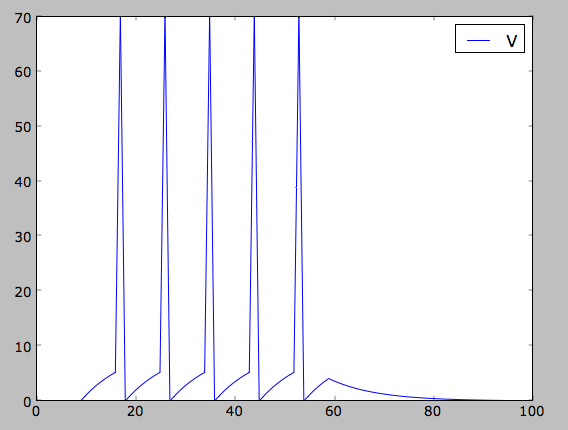
\includegraphics[scale=0.71]{integratefirespikes.png}
\vspace{5pt}

In the above figure there is no activity until the point at which stimulation is applied.  At that point it spikes at uniform intervals until the stimulus is removed, at which point it decays back to rest exponentially.  

\subsection{B. Amplitude Response}

The response of the model varies based on what amplitude of stimulus it receives.  The spiking always remains at consistent intervals over the range of amplitude values, but the rate of firing increases as the amplitude increases.  Under an amplitude of 0.6 nA the model fails to produce spikes at all.  From 0.6 to around 5 nA the rate of the firing increases, but saturates at 333 Hz.  Its ascent under the influence of higher firing rates reveals some artifacts of the integrate and fire model.

\vspace{15pt}
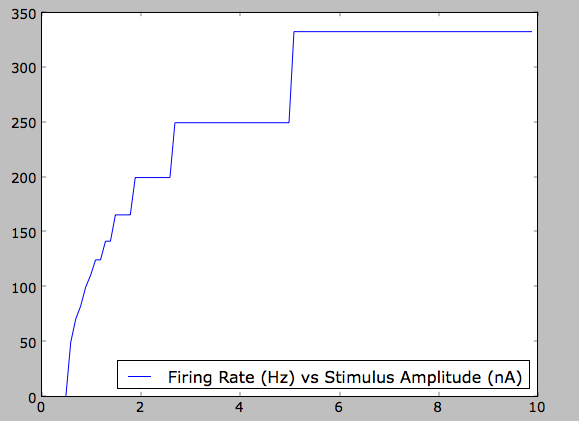
\includegraphics[scale=0.71]{integratefiretrials.png}
\vspace{5pt}

The sudden jumps are artifacts due to the definition of the model.  Because the integrate and fire model defines a spike to take a single time step and the reset to take one more, the limit of the rate is entirely dependent on the resolution of the time step applied to the model.  The theoretical maximum of this model is therefore three time steps:  One to rise to or above $V_{thr}$, one to spike, and one more to reset.  

This is what we see above 5 nA in this trial run.  At saturation the response takes three time steps, maxxing out at 333 Hz.  Below that are artifacts based on stimulus amplitudes that take two time steps to reach threshhold, for instance, or three.  The curve evens out far from saturation, and could be considered reasonably well-behaved under 1 nA.  Still, this behavior is a severe limitation of the model, and should be taken under heavy consideration whenever it is applied.

\section{Spike-Response Models - Analysis}



\section{Poisson Spikes}

If a spike train is generated from a poisson process with a time dependent firing rate, there must be some way to get that firing rate back from the spike train alone.  One method is to approximate the firing rate as the integration of an exponential decay function for each spike.  The key parameter here is the rate of decay, given by $\tau_{approx}$.  The whole approximation works as follows:

$$ \od{r_{approx}}{t}=\frac{-r_{approx}}{\tau_{approx}} \text{       if there is a spike,} $$
$$ \od{r_{approx}}{t}=\frac{1}{\tau_{approx}} \text{   otherwise} $$

A poisson spike train with a time dependent firing rate of 

$$ r(t)=100(1+cos(\frac{2\pi t}{300ms})) $$

produces a random train of spikes with a distribution that maps to this firing rate.  If the approximation method is applied to the resulting spike train with a range of $\tau_{approx}$ from 1 to 100 and the error calculated as the difference between the true rate and the approximated rate squared, we get a variety of approximations more or less effective at reproducing the original rate that generated the spikes in the first place.  Taking the $\tau_{approx}$ with the minimum error, in this case $\tau_{approx}=24$ with an error squared of 3.22, we can compare all of this simultaneously.

\vspace{15pt}
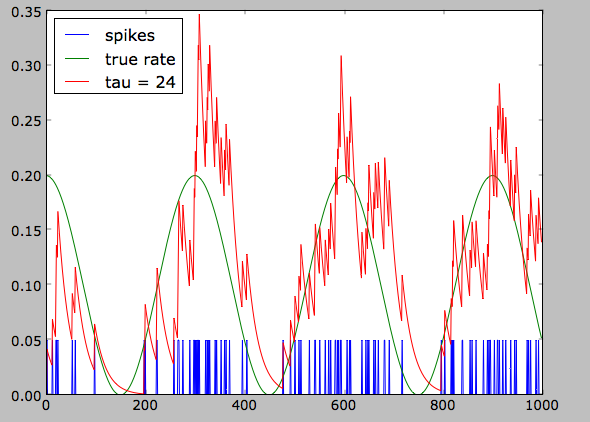
\includegraphics[scale=0.71]{poissonapprox.png}
\vspace{5pt}

A truly splendid graph.  The true rate is a cosine curve, and the rate of spike generation conforms to this curve.  This approximation in red is the one with the lowest error squared of all the trials $\tau_{approx}=1...100$

\end{document} 
